\documentclass[11pt,a4paper]{article}
\usepackage[utf8]{vietnam}
\usepackage{fontenc}
\usepackage{amsmath}
\usepackage{amsfonts}
\usepackage{amssymb}
\usepackage{graphics}
\usepackage{enumitem}
\usepackage{fancyhdr}
\usepackage{xcolor}
\usepackage{mdframed}
\usepackage{colortbl}
\usepackage{fontawesome}
\usepackage{tikz}
\usepackage{setspace}
\usepackage{listings}
\definecolor{dgray}{gray}{0.35} % colour of R comments
\definecolor{lgray}{gray}{0.9999} % background colour of R-code
\usetikzlibrary{patterns}
\usetikzlibrary{calc,angles}
\usepackage[left= 2cm, right = 2cm, top = 2cm, bottom = 2cm]{geometry}
\usepackage{scalefnt}
\usepackage{fancybox}
\usepackage{multirow}
\usepackage{pgfplots}
\usepackage{hyperref}
\definecolor{dkgreen}{rgb}{0,0.6,0}
\definecolor{gray}{rgb}{0.5,0.5,0.5}
\definecolor{mauve}{rgb}{0.58,0,0.82}
\pagestyle{fancy}
\fancyhf{}
%\rhead{\textit{Nhóm 18}}
\lhead{\textit{Bài Tập Lớn Đại Số Tuyến Tính}}
\lfoot{\textit{Nhóm 8-L16}}
\rfoot{Trang \thepage}
\renewcommand{\footrulewidth}{0.4pt}
\renewcommand{\headrulewidth}{0.4pt}
\lstset{ % setting appearance of R-code
	language=C, % setting language R
	basicstyle=\ttfamily\small, % font and size of R-code
	backgroundcolor=\color{lgray}, % background colour of R-code
	commentstyle=\ttfamily\small\itshape\color{dgray}, % colour of R comments
	showstringspaces=false, % forbidding the highlighting of spaces
	 % numbering on the left
	 % cumulative numbering of rows in consecutive uses of lstlisting environment
	breaklines=T} % automatic line breaks of code at the end of a line
\newmdenv[linewidth=0.6pt,linecolor=black,skipabove=\topsep,skipbelow=\topsep,
leftmargin=-5pt,rightmargin=-5pt,
innerleftmargin=5pt,innerrightmargin=5pt]{mybox}
\setlist{nolistsep}
\newcommand\tab[1][0.7cm]{\hspace*{#1}}
\setlength{\parindent}{0pt}
\begin{document}
\begin{titlepage}
	\begin{center}
		ĐẠI HỌC QUỐC GIA THÀNH PHỐ HỒ CHÍ MINH\\
		TRƯỜNG ĐẠI HỌC BÁCH KHOA\\
		KHOA KHOA HỌC ỨNG DỤNG\\
	\end{center}
	\begin{figure}[h!]
\begin{center}
\vspace{0.5cm}

\includegraphics[width=3cm]{hcmut.png}
\end{center}
\end{figure}
	\vspace{2cm}
	\begin{center}
		\begin{tabular}{c}
			\textbf{{\Large BÀI TẬP LỚN ĐẠI SỐ TUYẾN TÍNH}}\\ \\
			\hline
			\\ \\
			\textbf{\huge{\textcolor{blue}{PHÂN TÍCH A=QR BẰNG}}} \\
			\textbf{\huge{\textcolor{blue}{PHÉP BIẾN ĐỔI HOUSEHOLDER}}} \\
			\\ \\
			\hline
		%	\textbf{{\Large NHÓM 18}}\\ \\
		\end{tabular}
	\end{center}
	\vspace{3cm}
	
	\begin{table}[h]
\begin{tabular}{rrl}
\hspace{5 cm} & \textbf{Giảng viên hướng dẫn}: &Nguyễn Xuân Mỹ\\

& \textbf{Sinh viên thực hiện}: & Trần Minh Nhật  -- 2014008\\

%& & Trương Gia Hy  -- 2111427  \\
%& & Lê Vĩnh Khang  -- 2113661 \\
%& & Nguyễn Duy Khang  -- 2113666 \\
%& & Phạm Duy Khang  -- 1812556 \\
%& & Nguyễn Tuấn Khanh  -- 2110251 \\
%& & Huỳnh Gia Khiêm  -- 2113736 \\
\end{tabular}
\end{table}
	\vspace{3cm}
	\begin{center}
		{\footnotesize Ho Chi Minh City, 2022}
	\end{center}
\end{titlepage}
\newpage

\tableofcontents

\newpage
\section{CƠ SỞ LÍ THUYẾT PHÂN TÍCH A=QR BẰNG BIẾN ĐỔI HOUSEHOLDER}
\subsection{GIỚI THIỆU THUẬT TOÁN A=QR}
\subsubsection{Khái niệm phân rã QR} Trong đại số tuyến tính, phân rã $QR$, còn được gọi là phân
tích nhân tố $QR$ hoặc phân tích nhân tố $QU$ là phân rã ma trận $A$ thành tích $A = QR$
của ma trận trực giao $Q$ và ma trận tam giác trên $R$. Phân rã $QR$ thường được sử dụng
để giải quyết vấn đề bình phương tối thiểu tuyến tính và là cơ sở cho một thuật toán
eigenvalue cụ thể, thuật toán $QR$.

\subsubsection{Ý tưởng của thuật toán QR}
\begin{figure}[!ht]
	\centering
	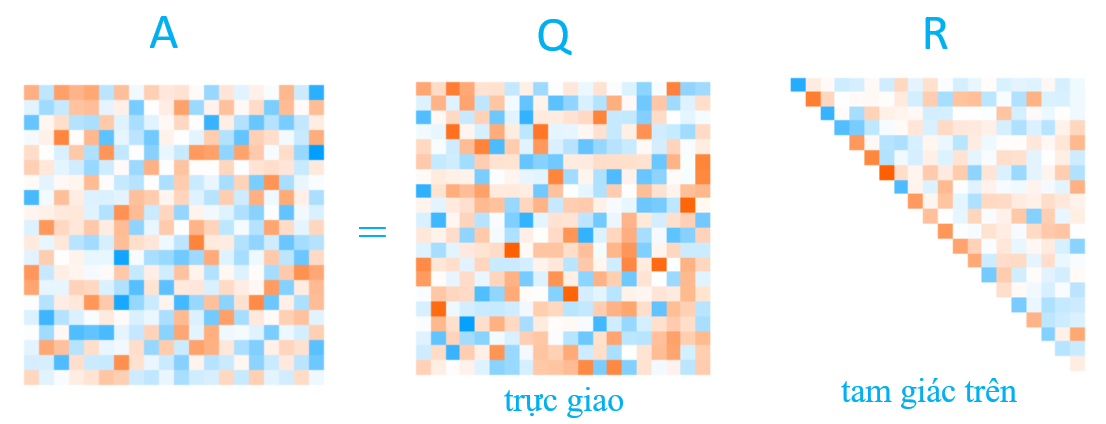
\includegraphics[scale=0.4]{ytuong}
	%\caption{\textit{Conversion between human, high-level, assembly, and machine language}}\label{fig:Picture}
\end{figure}

\subsubsection{Quy trình Gram-Schmidt}
Phân hủy QR có công thức sau: \\
\begin{center}
	$A=QR$
\end{center}
Trong đó:
\begin{itemize}
	\item A là ma trận ban đầu muốn phân rã
	\item Q là ma trận trực giao
	\item R là ma trận tam giác trên 
\end{itemize}
\begin{figure}[!ht]
	\centering
	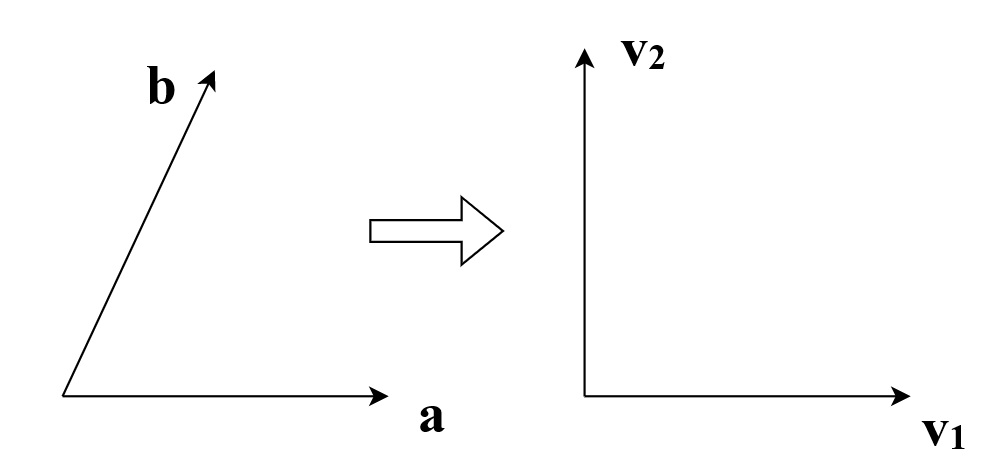
\includegraphics[scale=0.33]{dk}
	\caption{\textit{Trực giao các vector}}\label{fig:Picture}
\end{figure}
Điều kiện:\\
- Họ các véctơ cột của A là họ độc lập tuyến tính\\
- Dùng quá trình trực giao hóa Gram-Schmidt ta được họ trực giao và chia mỗi véctơ cho độ dài của nó ta có họ trực chuẩn. \\
- Ma trận trực giao $Q$ có các cột là véctơ trực chuẩn vừa tìm được. \\
- Ma trận $R$ (ma trận chuyển cơ sở từ $Q$ sang $E$) = $Q^{T}A$\\
Để tạo vectơ trực giao, chúng ta có thể sử dụng thông tin sau. Vectơ a là vectơ đầu tiên
và chúng ta có thể so khớp nó với $v_1$. $v_2$ phải trực giao với vectơ $v_1$, vì vậy chúng ta 
nên chiếu vectơ b lên $v_2$ để b trực giao với a ($v_1$). Phép chiếu của vectơ b lên a ($v_1$) 
được cho bởi:\\
\begin{center}
	$\dfrac{v_1^{T}b}{v_1^{T}v_1}v_1$
\end{center}

\begin{figure}[!ht]
	\centering
	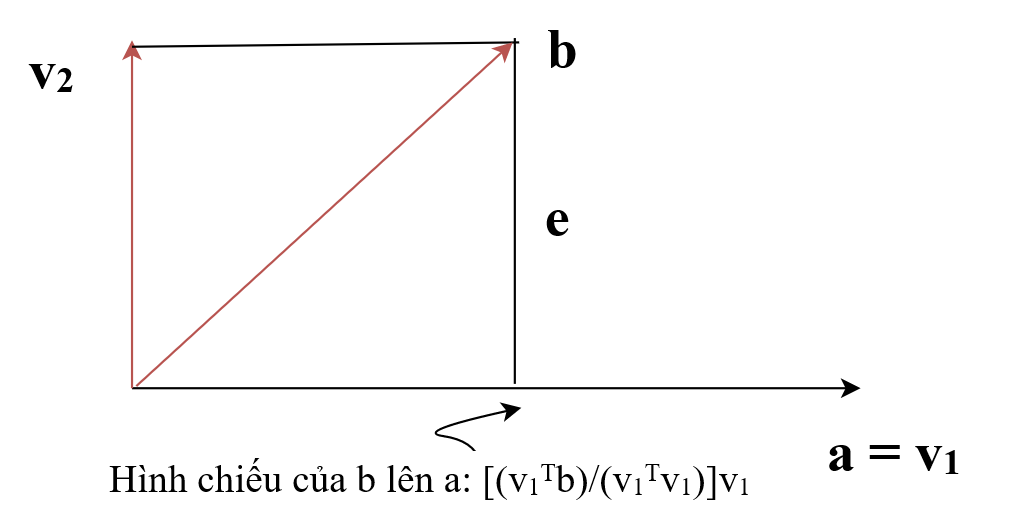
\includegraphics[scale=0.27]{hinhchieu}
	\caption{\textit{Phép chiếu vector}}\label{fig:Picture}
\end{figure}
Bây giờ chúng ta cần chiếu b lên $v_2$ để có được tính trực giao giữa a và b. Đối với điều 
này, chúng ta có thể sử dụng e, và có thể được tính bằng 
công thức sau:
\\
\begin{center}
	$e=b-\dfrac{v_1^{T}b}{v_1^{T}v_1}v_1$
\end{center}
Cần lưu ý là e có cùng độ dài và cùng chiều với $v_2$. Nên chúng ta có thể kết luận:\\
\begin{center}
	$v_2=b-\dfrac{v_1^{T}b}{v_1^{T}v_1}v_1$
\end{center}
Về cơ bản đây là cách hoạt động của quá trình Gram-Schmidt. Đối với nhiều hơn hai 
chiều (giả sử chúng ta có vectơ a, b và c), chúng ta có thể tính toán quá trình theo cách 
sau :\\
\begin{center}
	$v_3=c-\dfrac{v_1^{T}c}{v_1^{T}v_1}v_1-\dfrac{v_2^{T}c}{v_2^{T}v_2}v_2$
\end{center}

Để tính toán ma trận $R$, ta có thể biến đổi công thức $QR$:\\
\begin{center}
	$A=QR$\\
	$Q^{T}A=Q^{T}QR $ (vì Q trực giao nên $Q^{T}=Q^{-1})$\\
	$Q^{T}A=R$, do đó $R=Q^{T}A$
\end{center}
\subsubsection{Phản chiếu Householder}
Gram-Schmidt có thể không ổn định về mặt số học, có nghĩa là đầu vào thay đổi nhỏ 
có thể dẫn đến thay đổi tương đối lớn trong đầu ra ( nguồn ). Cách ổn định hơn là sử dụng phản chiếu của Householder. Householder chiếu vectơ qua một “tấm gương”. 
Chúng ta có vectơ $x$ mà chúng ta muốn phản ánh vectơ Qx. Để phản ánh, chúng ta sẽ 
sử dụng ma trận trực giao $Q$\\
\begin{figure}[!ht]
	\centering
	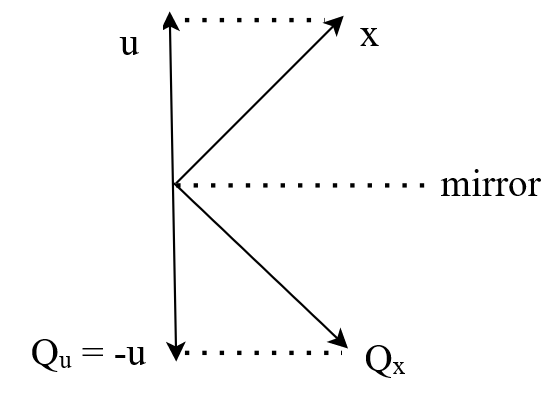
\includegraphics[scale=0.27]{mirror}
	\caption{\textit{Phản chiếu Householder}}\label{fig:Picture}
\end{figure}
Nội dung phản ánh\\
Từ trước, chúng ta biết rằng hình chiếu x lên u là:\\
\begin{center}
	$\dfrac{u^{T}x}{u^{T}u}u$
\end{center}
Từ biểu đồ phản chiếu của Householder, chúng ta có thể thấy rằng nếu chúng ta lấy x trừ đi hai lần thành phần song song với u, chúng ta sẽ nhận được Qx:\\
\begin{center}
	$Qx=x-2x_{||}$
\end{center}

Thành phần song song là hình chiếu x của chúng ta với u, vì vậy chúng ta có thể viết:\\

\begin{center}
	$Qx=x-2\dfrac{u^{T}x}{u^{T}u}u$
\end{center}

Vì tính kết hợp của phép nhân ma trận:\\
\begin{center}
	$u(u^{T}x)=(uu^{T})x$
\end{center}
Có thể viết:\\
\begin{center}
	$Qx=(uu^{T})x-2\dfrac{uu^{T}}{u^{T}u}x$
\end{center}
trở thành\\
Có thể viết:\\
\begin{center}
	$Qx=(I-2\dfrac{uu^{T}}{u^{T}u})x$
\end{center}
Cuối cùng ta có công thức sau:\\
\begin{center}
	$Q=I-2\dfrac{uu^{T}}{u^{T}u}$
\end{center}

\subsection{Lí thuyết và thuật toán}
\subsubsection{Đối với ma trận vuông}
Bất kì ma trận vuông thực A có thể phân tách thành: $A = QR$\\
Trong đó:\\
- Q là một ma trận trực giao (các cột của nó là các vectơ đơn vị trực giao, có 
nghĩa là $Q^{T}Q = QQ^{T}= 1$) \\
- R là ma trận tam giác trên (còn gọi là ma trận tam giác vuông)\\
Nếu A là khả nghịch, thì việc phân tích này là duy nhất nếu chúng ta yêu cầu các phần
tử đường chéo của R dương. Nếu thay vào đó A là một ma trận vuông phức, thì có một
phép phân tách $A = QR$, trong đó Q là một ma trận đơn vị (vì vậy Q*Q = QQ* = 1).\\
Nếu A có n cột độc lập tuyến tính, thì n cột đầu tiên của Q tạo thành cơ sở trực giao
cho không gian cột của A. Tổng quát hơn, các cột k đầu tiên của Q tạo thành cơ sở
trực giao cho nhịp của các cột k đầu tiên của A cho bất kì $1 \leq k \leq n$. Thực tế là bất kì
cột k nào của A chỉ phụ thuộc vào các cột k đầu tiên của Q chịu trách nhiệm cho dạng
tam giác của R.
\\
\subsubsection{Đối với ma trận hình chữ nhật}
Nói chung, chúng ta có thể tính đến một ma trận m×n phức tạp A, với $m \geq n$, là tích
của ma trận đơn nhất M × m Q và ma trận hình tam giác trên m × n R. Vì các hàng dưới
cùng $(m−n)$ của ma trận hình tam giác trên m × n bao gồm hoàn toàn các số không, nó
thường hữu ích cho phân vùng R hoặc cả R và Q:

\begin{center}
	\begin{center}
		$A=QR=Q
		\begin{bmatrix}
			R_1\\
			0\\
		\end{bmatrix}=[Q_1, Q_2]
		\begin{bmatrix}
			R_1\\
			0\\
		\end{bmatrix}=Q_1R_1
	\end{center}
\end{center}
Trong đó: $R_1$ là n × m ma trận tam giác trên, 0 là ma trận 0 (m – n) × n, $Q_1$ là m × n,
$Q_2$ là m × (m – n), $Q_1$ và $Q_2$ đều có cột trực giao.
\\

\begin{figure}[!ht]
	\centering
	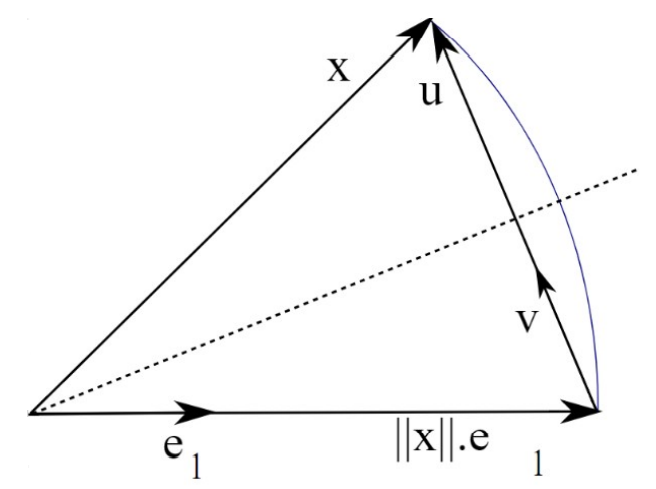
\includegraphics[scale=0.27]{non}
	%\caption{\textit{Phản chiếu Householder}}\label{fig:Picture}
\end{figure}

Phản chiếu Householder để phân rã QR: Mục tiêu là tìm một phép biến đổi
tuyến tính thay đổi vectơ x thành vectơ cùng độ dài và cùng phương với $e_1$. Chúng ta	
có thể sử dụng phép chiếu trực giao (Gram-Schmidt) nhưng điều này sẽ không ổn định
về mặt số nếu các vectơ x gần với trực giao. Thay vào đó, phản xạ của Householder
phản ánh qua đường đứt khúc (được chọn để chia đôi góc giữa x và $e_1$). Góc tối đa với
phép biến đổi này là $45^o$.\\
\subsubsection{Thuật toán phép biến đổi Householder}
Giả sử $u$ là vectơ khác không tùy ý, khi đó hình chiếu vuông góc của vectơ $v$ lên
không gian con $F$ sinh bởi vectơ $u$ là $pr_u(v) = uu^{T}v$.\\
Vectơ $v$ được phân tích thành $v = a + b$, với $a$ là hình chiếu vuông góc của $u$ lên $F$ và $b$
là hình chiếu vuông góc của $v$ lên $F$.\\
Ta có:\\
\begin{center}
	$\overrightarrow{ON}=\overrightarrow{OH}+\overrightarrow{HN}$ $\Rightarrow$ $y=\overrightarrow{ON}=(I-\dfrac{uu^{T}}{u^{T}u})v-\dfrac{uu^{T}}{u^{T}u}v=(I-2\dfrac{uu^{T}}{u^{T}u})v$
\end{center}

Vậy ta có phép đối xứng qua $F^{\bot}$ là $I-2\dfrac{uu^{T}}{u^{T}u}$
(phép biến đổi này được gọi là phép
biến đổi Householder)\\
\textbf{\textcolor{blue}{Cách thực hiện}}\\
Giả sử $A_{*1} \neq 0$ là cột thứ nhất của ma trận A.\\
Ta cần tìm một ma trận trực giao $P_1$ để $P_1A_{*1}=$
\begin{pmatrix}
	\vdots\\
	0\\
	\vdots\\
	0
\end{pmatrix}
Ma trận $P_1$ tương ứng với phép biến đổi trực giao nên nó bảo toàn độ dài của
vectơ. Vậy độ dài của $P_1A_{*1}$ bằng độ dài của $A_{*1}$.\\
Do đó, ta chọn $P_1A_{*1} = || A_{*1} ||e_1$.
\\
Đặt vector $\overrightarrow{OM}=A_{*1}$ và $\overrightarrow{ON}=|| A_{*1} ||e_1$. Khi đó 
$\overrightarrow{OM}=\overrightarrow{ON}+\overrightarrow{NM}$
$\Rightarrow$ $\overrightarrow{NM}=\overrightarrow{OM}-\overrightarrow{ON}$.\\
Đặt $u=\overrightarrow{NM}=A_{*1}-|| A_{*1} ||e_1$\\
Dùng vectơ u
này tạo ra phép biến đổi Householder $P_1=I-2\dfrac{uu^{T}}{u^{T}u}$ và phép biến
đổi này sẽ khử tất cả các phần tử trong cột thứ nhất cảu ma trận A ngoại trừ
hạng tử đầu tiên 
\newpage 
\section{CHƯƠNG TRÌNH MATLAB }
\subsection{Chương trình phân tích A=QR}
\begin{lstlisting}
	function [Q,R] = qr(A)
	% Phan tich QR cua ma tran A (mxn) dung
	% bien doi Householder 
	A=input('nhap A:');
	[m,n] = size(A);
	Q = eye(m); % Bien doi truc giao 
	R = A; % Ma tran da bien doi 
	for j = 1:n
	% -- Tim H = I-tau*w*wT de dat 0 vao duoi R(j,j)
	normx = norm(R(j:end,j));
	s = -sign(R(j,j));
	u1 = R(j,j) - s*normx;  
	w = R(j:end,j)/u1;
	w(1) = 1;
	tau = -s*u1/normx;
	% -- R := HR, Q := QH
	R(j:end,:) = R(j:end,:)-(tau*w)*(w'*R(j:end,:));
	Q(:,j:end) = Q(:,j:end)-(Q(:,j:end)*w)*(tau*w)';
	end
	disp('Q=');
	disp(-Q); % Dat -Q de ket qua giong voi tinh toan vi Q*R=(-Q)*(-R)
	disp('R=');
	disp(-R);
	
\end{lstlisting}

\subsection{Chương trình tính R và $Q^{T}b$}
\begin{lstlisting}
	function [Q,R] = lec18hqr1(A)
	% Compute the QR decomposition of an m-by-n matrix A using
	% Householder transformations.
	A=input('nhap A:');
	[m,n] = size(A);
	B=input('Nhap B:');
	Q = eye(m); % Orthogonal transform so far
	R = A; % Transformed matrix so far
	for j = 1:n
	% -- Find H = I-tau*w*w’ to put zeros below R(j,j)
	normx = norm(R(j:end,j));
	s = -sign(R(j,j));
	u1 = R(j,j) - s*normx;
	w = R(j:end,j)/u1;
	w(1) = 1;
	tau = -s*u1/normx;
	% -- R := HR, Q := QH
	R(j:end,:) = R(j:end,:)-(tau*w)*(w'*R(j:end,:));
	Q(:,j:end) = Q(:,j:end)-(Q(:,j:end)*w)*(tau*w)';
	end
	R=R
	QTb=Q'*B'
	
\end{lstlisting}
\newpage 
\subsection{Ví dụ minh họa}
\textbf{\textcolor{red}{Ví dụ 1}}\\
Cho ma trận $A=$
\begin{bmatrix}
	12 & -51 & 4\\
	6 & 167 & -68\\
	-4 & 24 &-41\\
\end{bmatrix}
Đầu tiên, chúng ta cần dùng phép phản chiếu để biến đổi cột đầu tiên của ma 
trận A, vector $a_1=$
\begin{bmatrix}
	12 & 6 & -4
\end{bmatrix}$^\intercal$ thành $|| a_1||e_1=$
\begin{bmatrix}
	\alpha & 0 & 0
\end{bmatrix}$^\intercal$\\
Ta có:

\begin{center}
	$u=x-\alpha e_1$;	$v=\dfrac{u}{||u||}$\\
	Với $\alpha=14$ và  $x=a_1=$
	\begin{bmatrix}
		12 & 6 & -4
	\end{bmatrix}$^\intercal$\\
\end{center}
Do đó:\\
\begin{center}
	$u=$
	\begin{bmatrix}
		-2 & 6 & -4
	\end{bmatrix}$^\intercal$=2\begin{bmatrix}
		-1 & 3 & -2
	\end{bmatrix}$^\intercal$\\ và 
	$v=\dfrac{1}{\sqrt{14}}$\begin{bmatrix}
		-1 & 3 & -2
	\end{bmatrix}$^\intercal$\\
	$Q_1=I-\dfrac{2}{\sqrt{14}\sqrt{14}}$
	\begin{bmatrix}
		-1\\
		3\\
		-2
	\end{bmatrix}
	\begin{bmatrix}
		-1 & 3 & -2
	\end{bmatrix}$=I-\dfrac{1}{7}$
	\begin{bmatrix}
		1 & -3 & 2\\
		-3 & 9 & -6\\
		2 & -6 & 4\\
	\end{bmatrix}=
	\begin{bmatrix}
		6/7 &  3/7  & -2/7\\
		3/7 & -2/7 & 6/7\\
		-2/7 & 6/7 & 3/7\\
	\end{bmatrix}
\end{center}
Từ đây ta có:\\
\begin{center}
	$Q_1A=$
	\begin{bmatrix}
		14 & 21 & -14\\
		0 & -49 & -14\\
		0 & 168 & -77\\
	\end{bmatrix}
\end{center}
Chúng ta gần như đã có một ma trận tam giác, chúng ta chỉ còn cần biến đổi giá trị hàng 3 cột 2 thành giá trị 0.\\
Lấy ma trận (1, 1) phụ hợp, sau đó áp dụng lại quy trình cho \\
\begin{center}
	$A'=M_{11}=$
	\begin{bmatrix}
		-49 & -14\\
		168 & -77\\
	\end{bmatrix}
\end{center} 
Bằng phương pháp tương tự ở trên, ta có được ma trận của phép biến đổi 
Householder\\
\begin{center}
	$Q_2=$
	\begin{bmatrix}
		1 & 0 & 0 \\
		0 & -7/25 & 24/25\\
		0 & 24/25 & 7/25 \\
	\end{bmatrix}
\end{center}
Tiếp theo ta tính\\
\begin{center}
	$Q=Q_1^{T}Q_2^{T}$
	\begin{bmatrix}
		6/7 & -69/175 & 58/175 \\
		3/7 & 158/175 & -6/175\\
		-2/7 & 6/35 & 33/35\\
	\end{bmatrix}
\end{center}
Hoặc\\
\begin{center}
	$Q=Q_1^{T}Q_2^{T}$
	\begin{bmatrix}
		0.8571 & -0.3943 & 0.3314 \\
		0.4286 & 0.9029 & -0.0343\\
		-0.2857 & 0.1714 & 0.9429\\
	\end{bmatrix}
\end{center}
\begin{center}
	$R=Q_2Q_1A=Q^{T}A=$	
	\begin{bmatrix}
		14 & 21 & -14 \\
		0 & 175 & -70\\
		0 & 0 & -35\\
	\end{bmatrix}
\end{center}
\newpage 
\textbf{\textcolor{red}{MATLAB ví dụ 1}}\\
\begin{figure}[!ht]
	\centering
	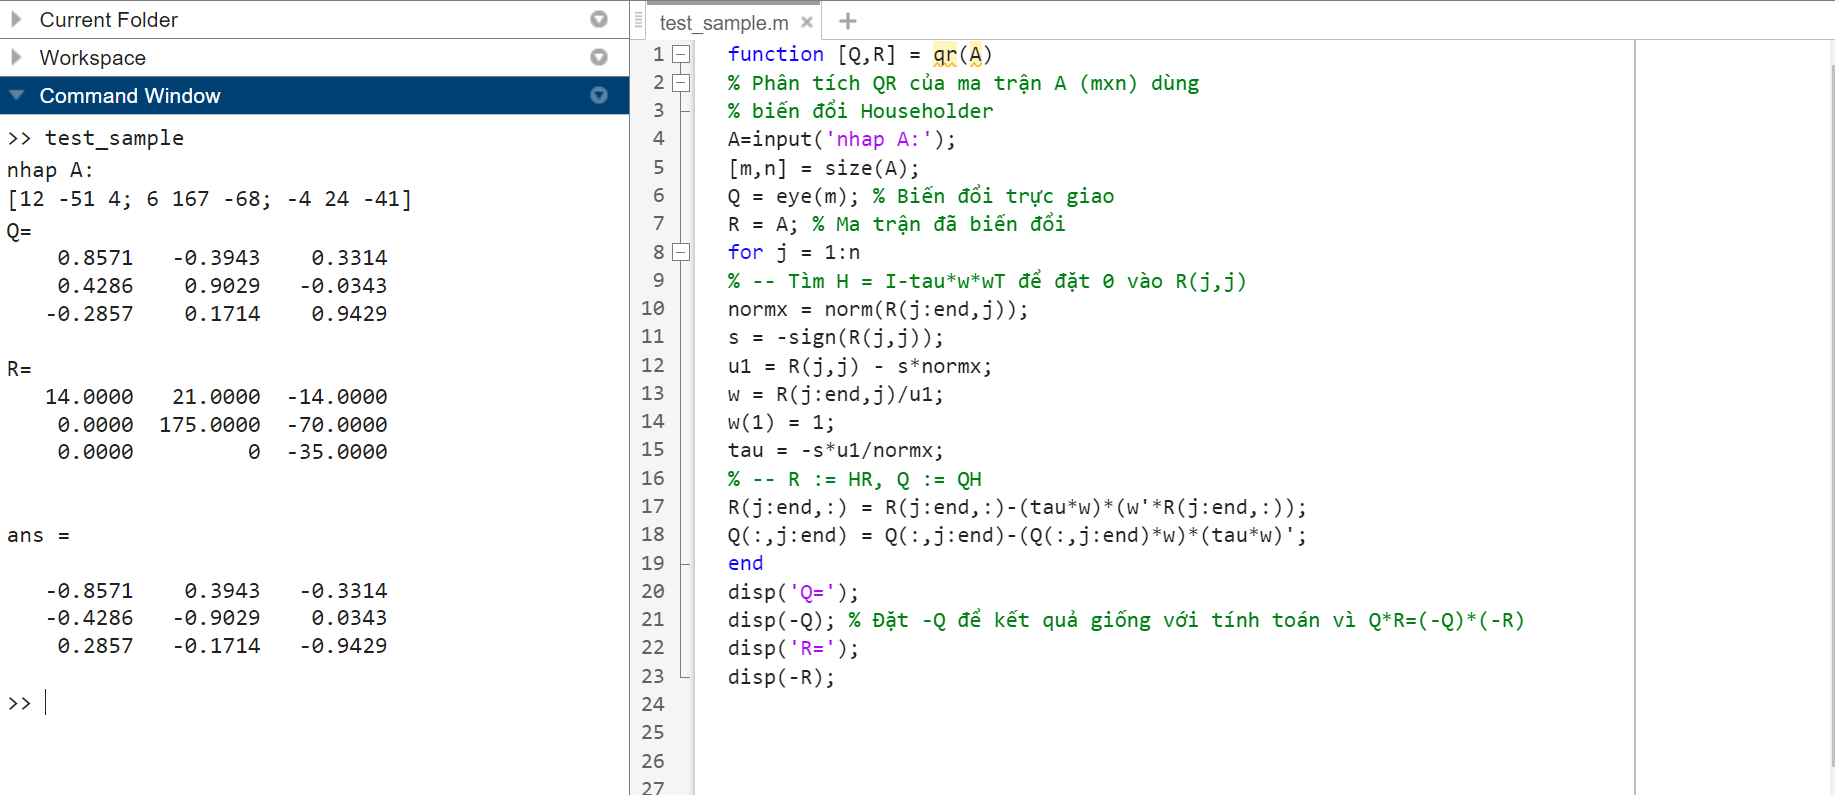
\includegraphics[scale=0.27]{code}
	%\caption{\textit{Phản chiếu Householder}}\label{fig:Picture}
\end{figure}
Nhận xét: kết quả của chương trình MATLAB giống với tính toán lí thuyết

\\
\textbf{\textcolor{red}{Ví dụ 2}}\\
Cho ma trận $A=$
\begin{bmatrix}
	1 & -1 & 4\\
	1 & 4 & -2\\
	1 & 4 & 2\\
	1 & -1 & 0\\
\end{bmatrix}
Đầu tiên, chúng ta cần dùng phép phản chiếu để biến đổi cột đầu tiên của ma 
trận A, vector $a_1=$
\begin{bmatrix}
	1 & 1 & 1 & 1
\end{bmatrix}$^\intercal$ thành $|| a_1||e_1=$
\begin{bmatrix}
	\alpha & 0 & 0 & 0
\end{bmatrix}$^\intercal$\\
Ta có:

\begin{center}
	$u=x-\alpha e_1$;	$v=\dfrac{u}{||u||}$\\
	Với $\alpha=2$ và  $x=a_1=$
	\begin{bmatrix}
		1 & 1 & 1 & 1
	\end{bmatrix}$^\intercal$\\
\end{center}
Do đó:\\
\begin{center}
	$u=$
	\begin{bmatrix}
		-1 & 1 & 1 & 1
	\end{bmatrix}$^\intercal$\\ và 
	$v=\dfrac{1}{2}$\begin{bmatrix}
		-1 & 1 & 1 & 1
	\end{bmatrix}$^\intercal$\\
	$Q_1=I-\dfrac{2}{2.2}$
	\begin{bmatrix}
		-1\\
		1\\
		1\\
		1
	\end{bmatrix}
	\begin{bmatrix}
		-1 & 1 & 1 & 1
	\end{bmatrix}$=I-\dfrac{1}{2}$
	\begin{bmatrix}
		1 & -1 & -1 & -1\\
		-1 & 1 & 1 & 1\\
		-1 & 1 & 1 & 1\\
		-1 & 1 & 1 & 1\\
	\end{bmatrix}=
	\begin{bmatrix}
		1/2 &  1/2  & 1/2 & 1/2\\
		1/2 &  1/2 & -1/2 &  -1/2 \\
		1/2 &  -1/2 & 1/2 &  -1/2 \\
		1/2 &  -1/2 & -1/2 &  1/2 \\
	\end{bmatrix}
\end{center}
Từ đây ta có:\\
\begin{center}
	$Q_1A=$
	\begin{bmatrix}
		2 & 3 & 2\\
		0 & 0 & 0\\
		0 & 0 & 4\\
		0 & -5 & 2\\
	\end{bmatrix}
\end{center}
Chúng ta gần như đã có một ma trận tam giác, chúng ta chỉ còn cần biến đổi giá trị hàng 3 cột 2 thành giá trị 0.\\
Lấy ma trận (1, 1) phụ hợp, sau đó áp dụng lại quy trình cho \\
\begin{center}
	$A'=M_{11}=$
	\begin{bmatrix}
		0 & 0\\
		0 & 4\\
		-5 & 2 \\
	\end{bmatrix}
\end{center} 
Bằng phương pháp tương tự ở trên, ta có được ma trận của phép biến đổi 
Householder\\
\begin{center}
	$Q_2=$
	\begin{bmatrix}
		1 & 0 & 0 & 0 \\
		0 & 0 & 0 & -1\\
		0 & 0 & 1 & 0 \\
		0 & -1 & 0 & 0\\ 
	\end{bmatrix}
\end{center}
Tiếp theo ta tính\\
\begin{center}
	$Q=Q_1^{T}Q_2^{T}$
	\begin{bmatrix}
		1/2 & -1/2 & 1/2 & 1/2 \\
		1/2 & 1/2 & -1/2 & -1/2\\
		1/2 & 1/2 & 1/2 & -1/2\\
		1/2 & -1/2 & -1/2 & -1/2 \\
	\end{bmatrix}
\end{center}
Hoặc\\
\begin{center}
	$Q=Q_1^{T}Q_2^{T}$
	\begin{bmatrix}
		0.5 & -0.5 & 0.5 & 0.5 \\
		0.5 & 0.5 & -0.5 & 0.5\\
		0.5 & 0.5 & 0.5 & -0.5\\
		0.5 & -0.5 & -0.5 & -0.5 \\
	\end{bmatrix}
\end{center}
\begin{center}
	$R=Q_2Q_1A=Q^{T}A=$	
	\begin{bmatrix}
		2 & 3 & 2 \\
		0 & 5 & -2\\
		0 & 0 & 4\\
		0 & 0 & 0 \\
	\end{bmatrix}
\end{center}

\textbf{\textcolor{red}{MATLAB ví dụ 2}}\\
\begin{figure}[!ht]
	\centering
	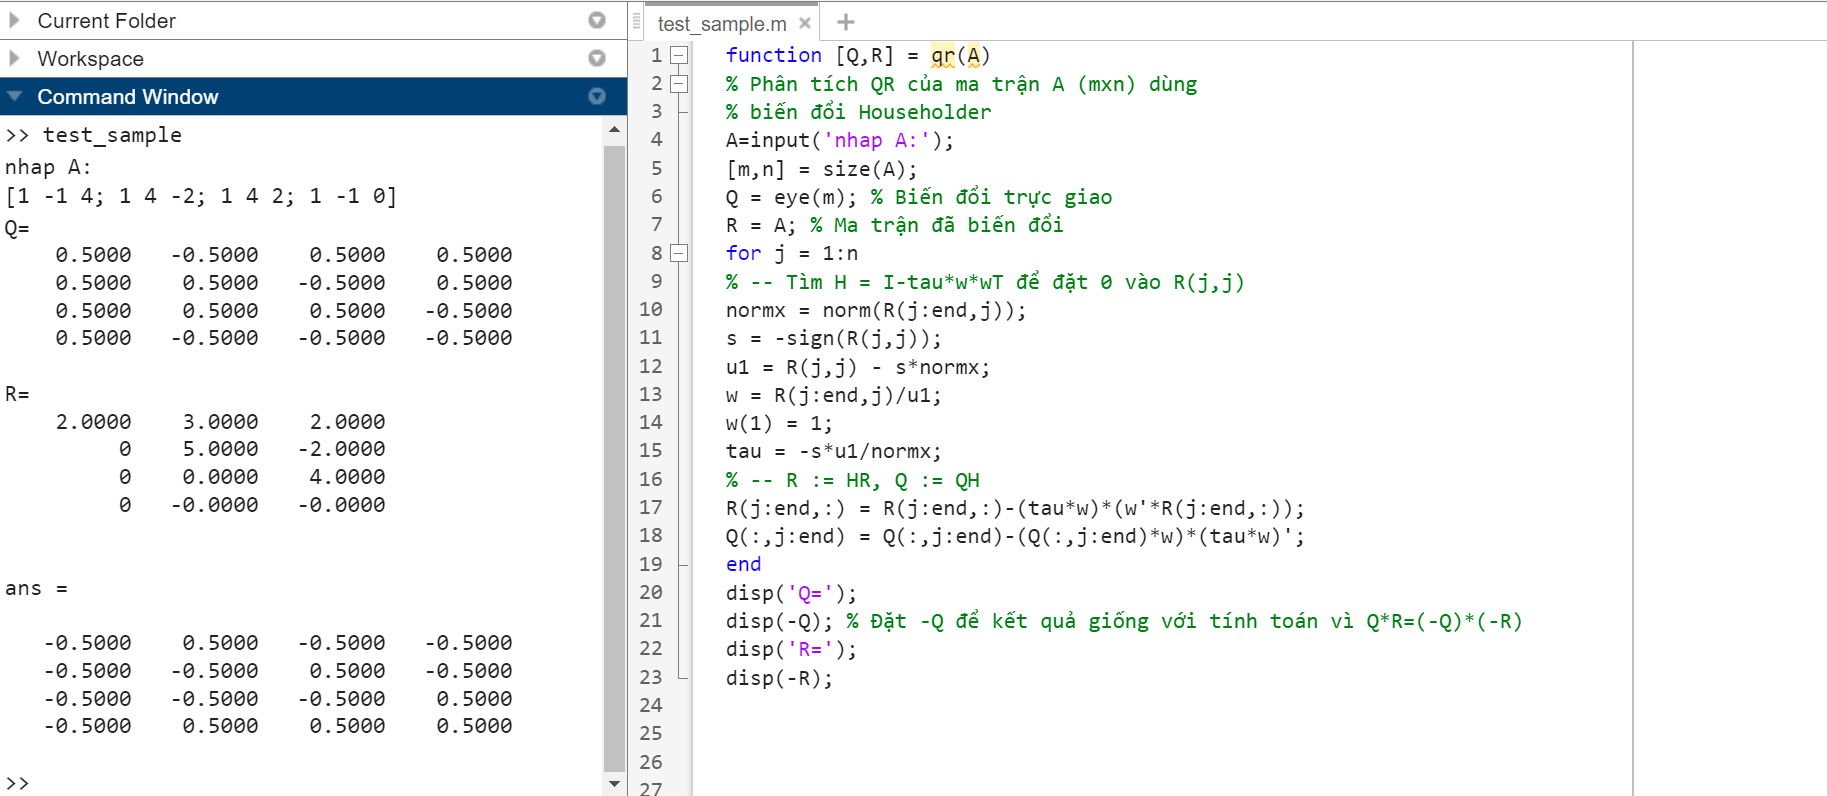
\includegraphics[scale=0.27]{code2}
	%\caption{\textit{Phản chiếu Householder}}\label{fig:Picture}
\end{figure}
Nhận xét: kết quả của chương trình MATLAB giống với tính toán lí thuyết

\newpage 
\section{Các ứng dụng của phép phân tích A = QR}
\subsection{Giải quyết các bài toán tìm giá trị riêng:}
\subsubsection{Các bước tìm trị riêng bằng phương pháp QR }
\begin{itemize}
	\item Tìm s từ ma trận A đã cho, ta có ma trận $A-\lambda i$ 
	\item Từ ma trận $A_k^{(i)}$ $\Rightarrow$ Ma trận quay $P_{k + 1}.$
	\item Tính $A_{k+1}^{(i)}$
	\item Tìm các giá trị riêng của ma trận A đã cho.
\end{itemize}
\subsubsection{Công thức cần lưu ý}
\begin{itemize}
	\item $A^{(i)}=Q^{(i)}R^{(i)}$ 
	\item $A^{(i+1)}=Q^{(i)}r^{(i)}$
	\item $A_2^{(1)}=P_2A^{(1)}$
	\item $A_3^{(1)}=P_3A^{(1)}_2$
	\item $A^{(2)}=R^{(1)}Q^{(1)}=P_3P_2A^{(1)}P_2'P_3'$
	\item Dạng tổng quát của $P_{k+1}$:\\
	\begin{center}
		\begin{figure}[!ht]
			\centering
			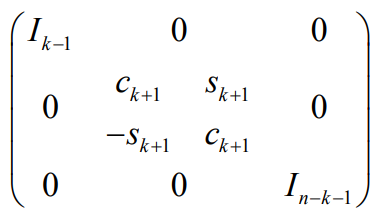
\includegraphics[scale=0.27]{matran}
			%\caption{\textit{Phản chiếu Householder}}\label{fig:Picture}
		\end{figure}
	\end{center}
	Với 
	\begin{center}
		$s_{k+1}=\dfrac{b_{k+1}}{\sqrt{b^2_{k+1}+x^2_k}}$; $c_{k+1}=\dfrac{x_k}{\sqrt{b^2_{k+1}+x^2_k}}$
	\end{center}
\end{itemize}
\subsubsection{Ví dụ}
Cho ma trận $A = $
\begin{bmatrix}
	3 & 1 & 0\\
	1 & 3 & 1\\
	0 & 1 & 3
\end{bmatrix} là ma trận 3 đường chéo, đối xứng. Tìm trị riêng của A?\\
\begin{center}
	\textbf{\textcolor{red}{Giải}}
\end{center}
- Tính $s_1$ bằng cách tìm trị riêng ma trận vuông 2 × 2 tạo bởi dòng thứ 2,3 và cột thứ 2,3 \\
\begin{center}
	\begin{bmatrix}
		3 & 1\\
		1 & 3\\
	\end{bmatrix}
\end{center}
Ma trận này có 2 trị riêng $\mu_1=2$ và $\mu_2=4$\\
Chọn trị riêng gần với giá trị $a_3 = A_{33} = 3$ $\Rightarrow$ Chọn $s_1 = \mu_1 = 2$\\
- Ta có:
\begin{center}
	$A^{(i)}=A-s_1I=$
	\begin{bmatrix}
		3 & 1 & 0 \\
		1 & 3 & 1 \\
		0 & 1 & 3 \\
	\end{bmatrix}-2
	\begin{bmatrix}
		1 & 0 & 0 \\
		0 & 1 & 0 \\
		0 & 0 & 1 \\
	\end{bmatrix}=
	\begin{bmatrix}
		1 & 1 & 0 \\
		1 & 1 & 1 \\
		0 & 1 & 1 \\
	\end{bmatrix}\\
	$\Rightarrow$ $x_1=1; b_2=1; s_2=c_2=\dfrac{\sqrt{2}}{2}$
\end{center}
\newpage 
- Dạng của $P_2$::
\begin{center}
	\begin{figure}[!ht]
		\centering
		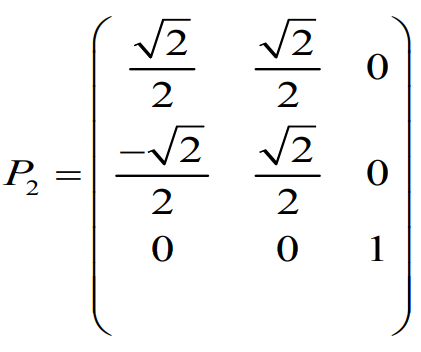
\includegraphics[scale=0.244]{p}
		%\caption{\textit{Phản chiếu Householder}}\label{fig:Picture}
	\end{figure}\\
	\begin{figure}[!ht]
		\centering
		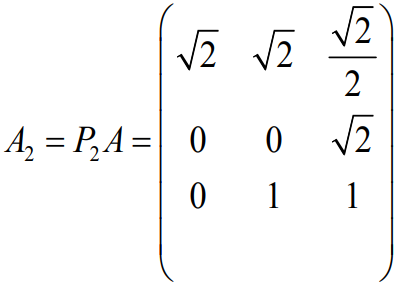
\includegraphics[scale=0.27]{aa}
		%\caption{\textit{Phản chiếu Householder}}\label{fig:Picture}
	\end{figure}\\
	$\Rightarrow$ $x_2=0$; $b_3=1$; $s_1=0$; $c_3=1$\\
\end{center}\\
- Dạng của $P_3$:
\begin{center}
	$P_3=$
	\begin{bmatrix}
		1 & 0 & 0 \\
		0 & 0 & -1\\
		0 & -1 & 0\\
	\end{bmatrix}
\end{center}
\\
- Ma trận $A^{(2)}=R^{(1)}Q^{(1)}=P_3P_2A_1^{(1)}P_2'P_3'=$
\begin{figure}[!ht]
	\centering
	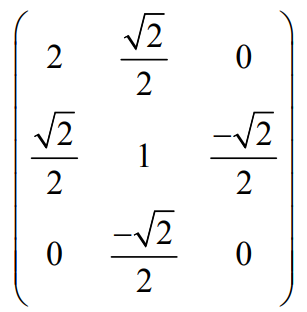
\includegraphics[scale=0.27]{aaa}
	%\caption{\textit{Phản chiếu Householder}}\label{fig:Picture}
\end{figure}\\
- Tương tự như trên ta có:
\begin{center}
	$s_2=\dfrac{1}{2}-\dfrac{\sqrt{3}}{2}$\\
	\\
	$A^{(3)}=$
	\begin{bmatrix}
		2.6720277 & 0.37597448 & 0\\
		0.37597448 & 1.4736080 & 0.030396964\\
		0 &  0.030396964 & -0.047559530 \\
	\end{bmatrix}
\end{center}
Nhận thấy $b_3^{(2)} = 0.030396964$ đã đủ nhỏ, ta đi tính các giá trị riêng:
\\
\begin{center}
	$\lambda=a_3^{(3)}+s_1+s_2=1.5894151$
\end{center}\\
- Bỏ đi hàng 3 cột 3 ma trận $A^{(3)}$, ta được:\\
\begin{center}
	\begin{bmatrix}
		2.6720277 & 0.37597448\\
		0.37597448 & 1.4736080 \\
	\end{bmatrix}
\end{center} \\
+ 2 trị riêng của ma trận trên là: $\mu_1 = 2.7802140$ và $\mu_2 = 1.3654218$\\
+ 2 trị riêng còn lại của ma trận A là:\\
\begin{center}
	$\lambda_1=\mu_1+s_1+s_2=4.4141886$\\
	$\lambda_2=\mu_2+s_1+s_2=2.9993964$\\
\end{center}
Ta dùng phép lặp (n = 20 lần ) cho đến khi các giá trị ngoài đường chéo chính hội tụ 
dần về 0 với chương trình \textbf{[Q,R] = qr(A)} được tạo như trên bằng thuật toán sau :\\
[Q, R]=qr(A)\\
A=Q*R\\
i=1:n\\
[Q,R]=qr($A_i$)\\
$A_{i+1}=R*Q$\\
So sánh với ma trận D chứa trị riêng nằm trên đường chéo chính được tạo bởi hàm
\textbf{[V,D] = eig(A)} trong matlab và kết quả của ví dụ trên ta thấy phép phân tích A=QR có thể sử dụng để tính trị riêng của ma trận với điều kiện lặp đủ số lần\\
\begin{figure}[!ht]
	\centering
	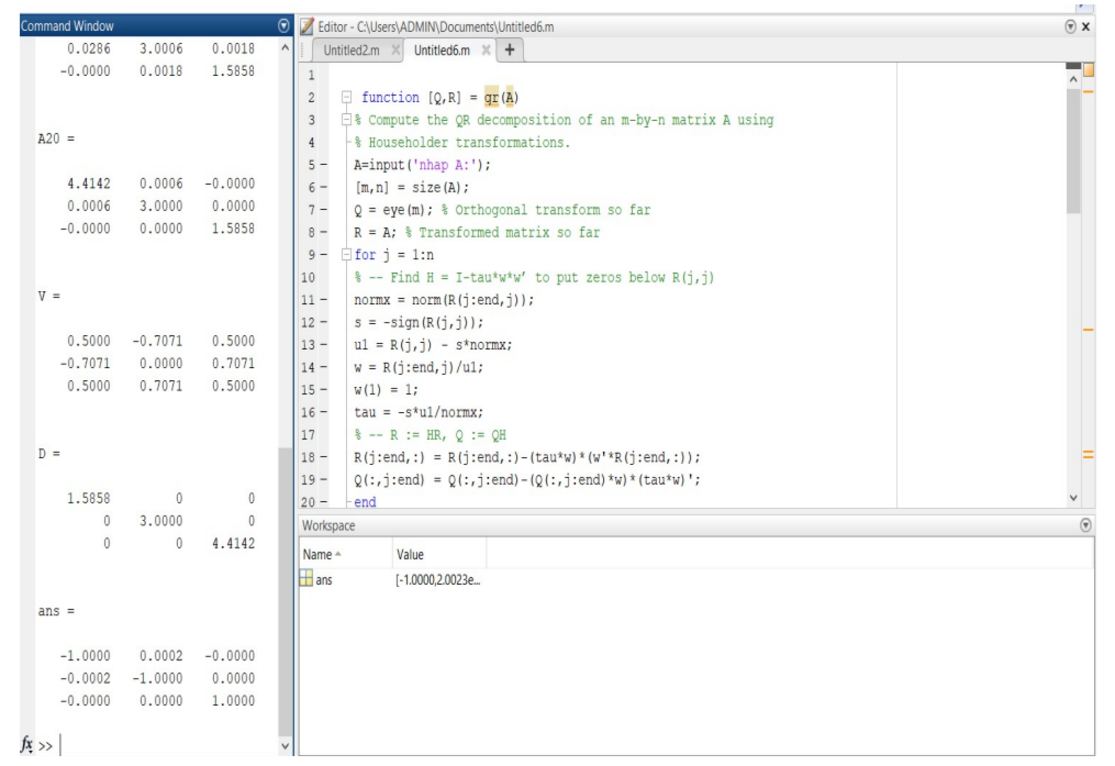
\includegraphics[scale=0.4]{ttt}
	%\caption{\textit{Phản chiếu Householder}}\label{fig:Picture}
\end{figure}\\
\subsection{Ứng dụng trong MIMO}
Trong radio, nhiều đầu vào và nhiều đầu ra, hay MIMO, là việc sử dụng nhiều ăng-ten
ở cả máy phát và máy thu để cải thiện hiệu suất truyền thông\\
\begin{itemize}
	\item MIMO là một trong nhiều dạng công nghệ ăng ten thông minh
	\item MIMO cung cấp sự gia tăng đáng kể về thông lượng dữ liệu và phạm vi liên kết
	mà không cần thêm băng thông hoặc công suất truyền
	\item MIMO là một phần quan trọng của các tiêu chuẩn truyền thông không dây hiện
	đại như IEEE 802.11n (Wifi) và 4G
	\item Trong hệ thống MIMO, một máy phát sẽ gửi nhiều luồng bằng nhiều ăng-ten
	phát. Các luồng truyền đi qua một kênh ma trận bao gồm tất cả các đường dẫn 
	$N_tN_r$ giữa các ăng ten phát $N_t$ ở máy phát và $N_r$ ăng-ten thu ở máy thu.
	
	\item Sau đó, máy thu nhận các vectơ tín hiệu đã nhận bởi nhiều ăng-ten thu và giải
	mã các vectơ tín hiệu nhận được thành thông tin ban đầu
	
\end{itemize}
\textbf{\textcolor{red}{Mô tả toán học}}\\

Cho $x = (x_1,..., x_n)^\intercal$ là một vectơ được truyền qua một kênh nhiễu.
Mỗi xi được chọn từ một bảng chữ cái có kích thước hữu hạn X
Một hệ thống MIMO chung được mô hình hóa như $r=Hx+\xi$\\
H là m × n kênh ma trận xếp hạng cột đầy đủ ($m \geq n$) (bộ thu đã biết)\\
$\xi = (\xi 1,...,\xi m)^\intercal$ là vectơ nhiễu Gaussian màu trắng trong đó $E(\xi\xi^{*})=\sigma2I$\\
$r=(r1,...,rm)^\intercal$ là vectơ nhận được quan sát.\\
Nhiệm vụ của chúng ta là phát hiện / ước lượng vectơ $x = (x_1,.., x_n)^\intercal$ $\in X_n$ với quan 
sát nhiễu r.\\
Sự phân hủy QR của ma trận kênh H có thể được sử dụng để tạo thành bộ dò hủy 
ngược.\\
Đặt $H = QR$, là phương trình phân rã QR của ma trận hệ thống H với m hàng, n cột.\\
Q = Ma trận trực giao m x n\\
R = Ma trận tam giác trên n x n\\
$\Rightarrow$ $r=Hx+\xi $ $\Rightarrow$ $Q*r=Rx+Q*\xi$\\
Đặt \begin{figure}[!ht]
	
	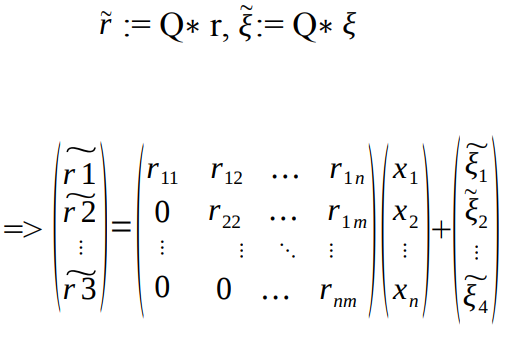
\includegraphics[scale=0.27]{uuu}
	%\caption{\textit{Phản chiếu Householder}}\label{fig:Picture}
\end{figure}\\
- Phương pháp chính thức:\\
Giả sử ước tính $xn$ bằng công thức: $xn:=Quant(t)$\\
Với $Quant(t)$ là phân tử X gần nhất với t\\
- Phân hủy \\
Công thức
\begin{center}
	$xn:=Quant(t)$\\
	$xk:=Quant[\dfrac{r_k-\Sigma r_{km}x_i}{r_{kk}}]$, $k=n-1, n-2,..., 1$
\end{center}
Về cơ bản thì đây là thuật toán bình phương cực tiểu
\\
Nhận xét:\\
- Sự phân rã QR cung cấp một cách thay thế để giải hệ phương trình $A x = b$ mà
không cần nghịch đảo ma trận A. Thực tế là Q là trực giao có nghĩa là $Q^{T}Q = I$,
do đó $A x = b$ tương đương với $R x = Q^{T}$
b, dễ giải hơn vì R là ma trận tam giác\\
- Việc sử dụng các phép biến đổi Householder vốn dĩ là đơn giản nhất trong số
các thuật toán phân rã QR ổn định về số lượng do sử dụng phản xạ làm cơ chế
tạo ra các số 0 trong ma trận R. Tuy nhiên, thuật toán phản chiếu Householder
nặng về băng thông và không thể song song hóa, vì mọi phản xạ tạo ra phần tử
0 mới sẽ thay đổi toàn bộ ma trận Q và R\\

\newpage 
\subsection{Giải quyết vấn đề bình phương cực tiểu}
Bình phương tối thiểu tuyến tính là một kỹ thuật trong ngành tối ưu toán học để 
tìm một nghiệm gần đúng cho một hệ phương trình tuyến tính không có nghiệm 
chính xác. Điều này thường xảy ra khi số phương trình là ($m$) lớn hơn 
số biến ($n$)\\
Theo từ ngữ toán học , chúng ta muốn tìm nghiệm của phương trình, với A là một ma trận cỡ m x n (với m > n) \\
Ta có: $A^{T}Ax=A^{T}b$ $\leftrightarrow$ $Rx=Q^{T}b$\\
Ví dụ: Tìm hàm bậc hai $f(t)=\alpha + \beta t + \gamma t^2$ với tập hợp $D={(2;7), (-2;8), (3;19), (-3;17)}$\\
Phương pháp:\\
Giả sử ta có tập hợp các điểm $D={(t_1;b_1),(t_2;b_2),…(t_m;b_m)}$. Cần tìm hàm $f=f(t)$ sao cho đồ thị của nó đi qua (hoặc gần nhất) tất cả các điểm của D\\
Xét trường hợp hàm $f(t)=\alpha +\beta g(t)+\gamma h(t)$\\
Tìm $\alpha, \beta, \gamma$ để $\epsilon(t) =\Sigma$ $(\alpha + \beta g(t_i)+\gamma h(t_i)-b_i)^2=\Sigma \epsilon^2_i$ nhỏ nhất. Phương pháp này gọi là bình phương cực tiểu\\
Ta tìm cực trị của hàm $\epsilon(t)$ có ba biến $\alpha, \beta, \gamma$. Để cho gọn , ta kí hiệu $g(t_i)=g_i$, $h(t_i)=h_i$\\
Điểm dừng của hàm $\epsilon(t)$ là\\

\begin{figure}[!ht]
	\centering
	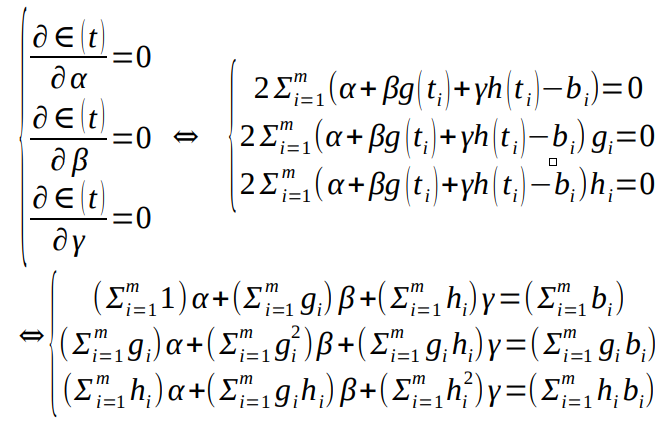
\includegraphics[scale=0.27]{eee}
	%\caption{\textit{Phản chiếu Householder}}\label{fig:Picture}
\end{figure}\\
Xét các ma trận 
\begin{figure}[!ht]
	\centering
	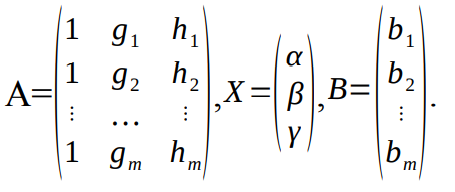
\includegraphics[scale=0.27]{ooo}
	%\caption{\textit{Phản chiếu Householder}}\label{fig:Picture}
\end{figure}\\
Hệ phương trình trên được ghi ở dạng ma trận $A^{T}Ã=A^{T}b$
Giải hệ phương trình trên ta được $\alpha, \beta, \gamma$ , suy ra $f(t )$.
Nếu $g(t)=t$ , $h (t )=0 $`, thì ta có đa thức bậc nhất $f (t )=\alpha + \beta t\\
Nếu $g(t)=t$, $h (t )=t^2$, thì ta có đa thức bậc hai $f(t )=\alpha+\beta t+$\gamma t^2$\\
Trong trường hợp tổng quát, ta có hàm $f (t )=\alpha_0+\alpha_1 g_1(t)+\alpha_2 g_2(t )+...+\alpha_n g_n(t)$ , ta làm 
tương tự. \\
\textbf{\textcolor{red}{Lời giải cho bài toán trên }}\\
Ta đặt $g(t)=t$, $h(t)=t^2$\\
Xét ma trận $A=$
\begin{bmatrix}
	1 & g1 & h1 \\
	1 & g2 & h2 \\
	1 & g3 & h3 \\
	1 & g4 & h4 \\
	
\end{bmatrix}=
\begin{bmatrix}
	1 & 2 & 4 \\
	1 & -2 & 4 \\
	1 & 3 & 9 \\
	1 & -3 & 9 \\
	
\end{bmatrix}, $b=$
\begin{bmatrix}
	7 \\
	8\\
	19\\
	17\\
	
\end{bmatrix}\\
Giải hệ phương trình $Rx=Q^{T}b$ (với R và $Q^{T}b$ như kết quả của chương trình). Ta được nghiệm $X=\Big(\dfrac{-9}{10};\dfrac{2}{13}; \dfrac{21}{10}\Big)^\intercal$ \\
Hàm cần tìm là $f(t)=\dfrac{-9}{10}+\dfrac{2}{13}t+\dfrac{21}{10}t^2$\\

\begin{figure}[!ht]
	\centering
	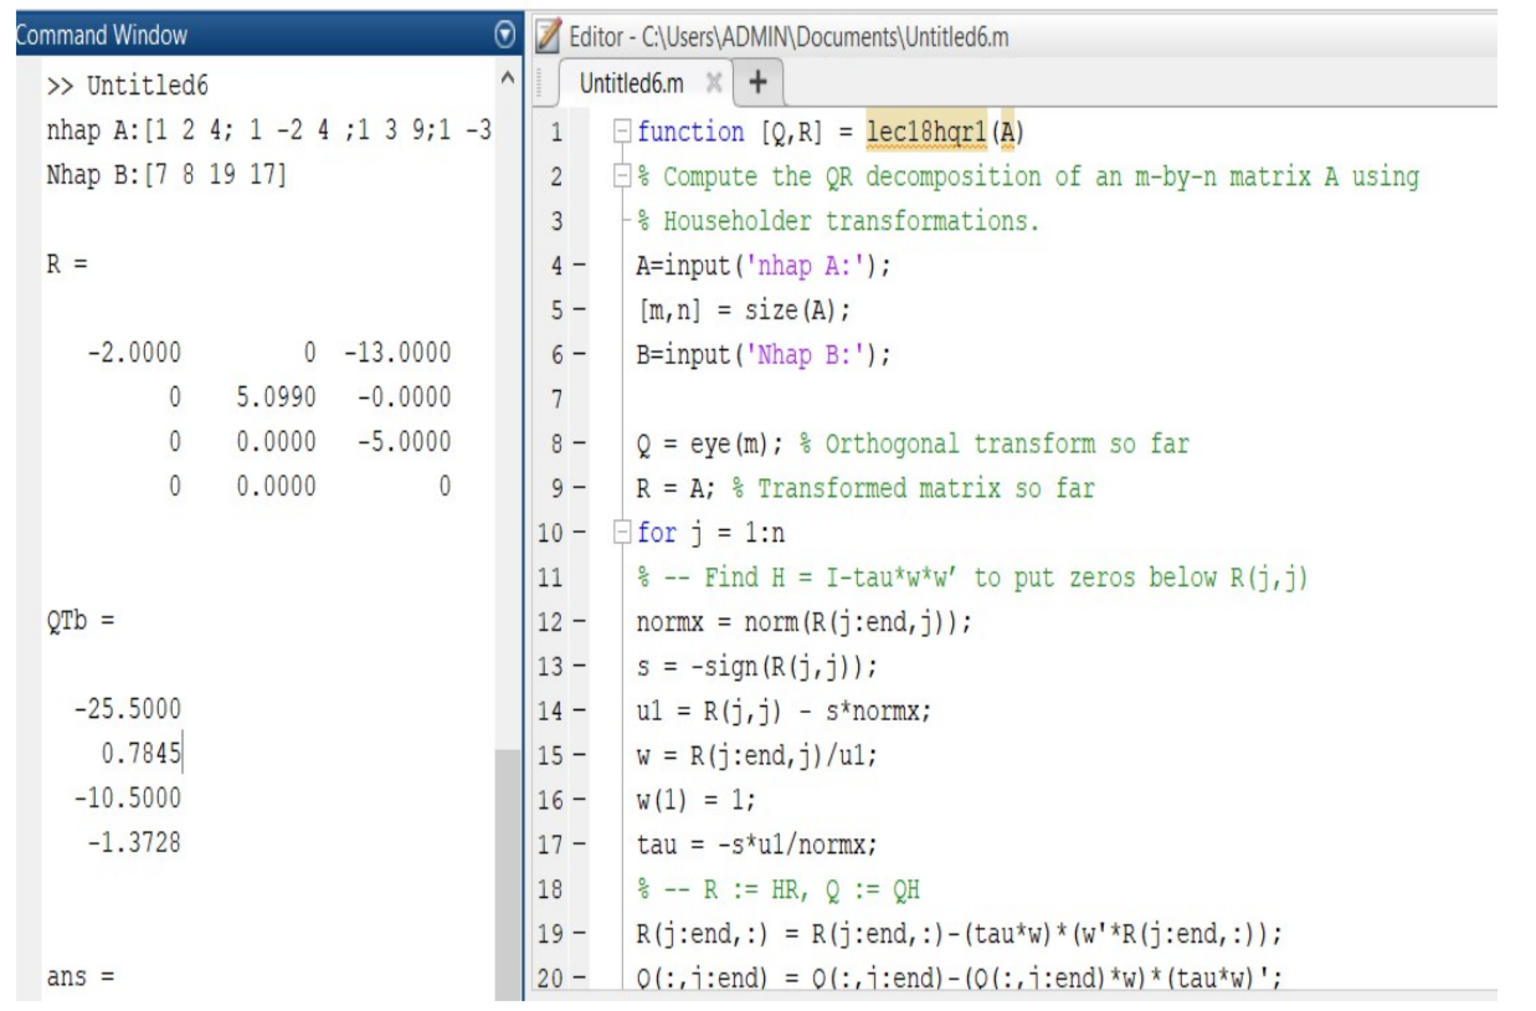
\includegraphics[scale=0.3]{yyy}
	%\caption{\textit{Phản chiếu Householder}}\label{fig:Picture}
\end{figure}

\newpage
\newpage 
\textfb{\textcolor{red}{Ví dụ 1}}\\













































\newpage 
%\addcontentsline{toc}{chapter}{Tài liệu tham khảo}
\begin{thebibliography}{99}
\bibitem{} Slideshare, {\it Tìm trị riêng bằng phương pháp QR}\\ \url{https://www.slideshare.net/PhanToanSimone/tm-tr-ring-bng-pp-qr}
\bibitem{} MATLAB Answers, {\it QR Factorization Using Householder Transformations}\\ \url{https://www.mathworks.com/matlabcentral/answers/169648-qr-factorization-using-householder-transformations}
\bibitem{} All MathWorks Blog, {\it Householder Reflections and the QR Decomposition}\\ \url{https://blogs.mathworks.com/cleve/2016/10/03/householder-reflections-and-the-qr-decomposition/}
\bibitem{} Youtube, {\it Householder Transformation with QR Decomposition Examples.}\\ \url{https://www.youtube.com/watch?v=OqgYYqy0M4w}

\bibitem{} WALTER GANDER, {\it Algorithms for the QR-Decomposition}\\ \url{https://people.inf.ethz.ch/gander/papers/qrneu.pdf}
\bibitem{} Tin-Yau Tam, {\it QR decomposition: History and its
	Applications}\\ \url{https://people.duke.edu/~hpgavin/SystemID/References/Tam-QR-history-2010.pdf}


\end{thebibliography}


\end{document}



















